%===================================== KAPITTEL 2 =================================

\chapter{Teori}
% Først, introduser og definer begrepet ''aggregatorientert datamodell'' - Kanskje jeg bør forklare ytterligere hva det betyr?
Ifølge \cite{sadalage2013} kan nøkkelverdi-lagre (eng. key-value store), kolonnefamilielagre (eng. column family stores) og dokumentlagre (eng. ''document stores'') ordnes under én og samme ''art'' av NoSQL-databaser: Aggregatorienterte databasesystem (eng. ''aggregate oriented databases''). Denne introduksjonen til de tre nevnte NoSQL - datamodellene forholder seg til denne klassifiseringen. Utover disse tre typene av NoSQL - modeller finnes også den graforienterte modellen, som benyttes av systemer som InfiniteGraph, OrientDB og FlockDB. Denne datamodellen vil ikke bli beskrevet i noen videre detalj. Det bør nevnes at med begrepet ''datamodell'' menes den programmatiske metoden data organiseres av et DBMS, i vitenskaplig notasjon er ''metamodell'' mer presist.

% Dette kapitlet presenterer litteraturoversikten og resultater fra prosjektarbeidet
Dette kapitlet gir leseren en innføring i tre NoSQL - datamodeller, hvordan de skiller seg ut fra den relasjonelle datamodellen, og hvordan deres forskjeller fra relasjonelle databaser har innvirkning på hvordan levende oppgradering av dem og migrasjon av eksisterende data i produksjonsmiljøet kan utføres i en smidig utviklingsprosess.

Vi begynner med å beskrive den relasjonelle datamodellen, og hvorfor den ikke holder mål i et distribuert produksjonsmiljø der større datavolum behandles. Dernest blir den aggregatorienterte datamodellen presentert, en kategori underordnet NoSQL-paraplyen som denoterer fellesnevneren mellom nøkkelverdilagre, dokumentlagre og kolonnefamilielagre. Samtlige tre former for aggregatorientering beskrives i avsnitt 2.2.1 til 2.2.3.

% Om den relasjonelle datamodellen
% Før første subseksjon: ; 2.1.3: Nøkkel-verdi-lagre; 2.1.4: Dokumentlagre; 2.1.5: KFL; 2.1.2 Ett eget overordnet kapittel om aggregatorientering; 2.1.1 mySQL?
% 2.1 - Om relasjonelle modeller, motivasjonen bak NoSQL
\section{Den relasjonelle datamodellen}

% Den relasjonelle datamodellen, i.e. MariaDB og Postgres (Bøyningen av sybstantivet 'tuppel' samsvarer med Bratsbergengens skrivemåte i hans artikkel om relasjonsdatabaser hos SNL)
For å forstå framveksten av NoSQL - databaser er . I den relasjonelle datamodellen organiseres forskjellige former for applikasjonsdata inn i relasjoner, og data tilhørende samme relasjon inndeles i atomiske, disjunkte enheter kalt \emph{tupler}. En tuppel er en flat, endimensjonal liste av dataverdier. Hver av disse verdiene korresponderer til nøyaktig ett attributt av relasjonen tuppelen er lagret i.

% Strukturelle begrensninger i relasjonsdatabaser
Det foreligger visse begrensninger på denne datastrukturen. Til eksempel kan ikke en enkelt tuppel nøstes inn i en annen, og hvert attributt i tuppelen har én atomisk korresponderende verdi, aldri en liste av verdier. Nå skal det sies at nyere versjoner av MariaDB støtter JSON-objekter som datatype \citep{mariadb}. JSON-objekter er serialiserte (dsv objekter konverterte til strenger), fleksible dataenheter som kan inneholde nøstede datastrukturer.

Imidlertid har ikke databasesystemet noen forståelse for de enkelte dataelementer som objektet innkapsler, det ser bare en helhetlig, ugjennomsiktlig dataenhet, nemlig verdien av ett attributt i relasjonen. Ettersom tupler er den minste, udelelige dataenheten i den relasjonelle modellen er det korrekt å fastslå at spørringer opererer med og returnerer (et helt antall) tupler for hver enkelt spørring \citep{sadalage2013}. Riktignok går det an å utvelge distinkte attributter i spørringen, også kjent som kommandoen \texttt{PROJECT} i relasjonell algebra, likefullt er den tellbare dataenheten i resultantrelasjonen tupler, også referert til som rader i kontekst av databaseapplikasjoner.

% Spørringsfleksibilitet (JOIN + avanserte operasjoner) - Fra databasepensum
Følgelig gir slike strengt strukturerte datamodeller stor fleksibilitet for spørringene som utføres av databasesystemet. Det kan for eksempel samle sammen alle verdier for ett spesifikt numerisk attributt i én bestemt relasjon, summere disse  attributtverdiene sammen og returnere resultatet som et separat attributt i resultanttuppelen. På samme vis kan relasjonsdatabasesystemet kalkulere gjennomsnittet for alle eller enkelte av tuplene i en relasjon, telle opp antallet tupler i den, finne den høyeste numeriske verdien eller finne den laveste.

Ved hjelp av JOIN-operasjoner finner man eksisterende tupler fra forskjellige relasjoner, relatert til hverandre via fremmednøkler, og resultanten av JOINen kan systemet også kalle disse aggregeringsoperasjonene på. NoSQL - databaser har ikke den samme fleksibiliteten til selv å utføre slike spørreoperasjoner: Hver spørring henter kun én dataenhet ad gangen, noe som holder især for nøkkelverdilagre. Hver spørring er logisk sett bare et oppslag på en nøkkel i en hashtabell. Eventuell aggregering der sum, gjennomsnitt eller ekstremalverdier regnes må gjøres i selve applikasjonen, etter at oppslag på \textbf{samtlige} nøkler er gjort i databasen.

% Figur 1
\begin{figure}[!ht]
    \centering
    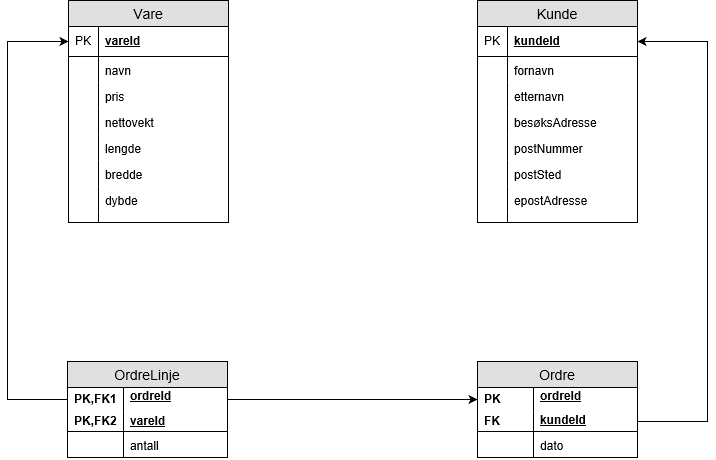
\includegraphics[scale=0.7]{fig/NettbutikkOrdreModell.png}
    \caption{Diagram over tabeller i en relasjonsdatabase som registrerer ordrer fra kunder i en netthandelapplikasjon.}
    \label{fig1}
\end{figure}
 
\subsection{Impedansproblemet (Impedance mismatch problem)}

I en typisk netthandelapplikasjon er applikasjonens datamodell denotert i form av dataobjekter midlertidig lagret i primærminnet, mer presist sagt, i adresseområdet til èn, eller flere, av nettleserens kjørende prosesser i kundens datamaskin. Variablene i datafeltene i disse objektene kan være saå mangt: strenger, tall, referenser til andre objekter, lister bestående av ovennevnte typer. Disse dataobjektene endres i sanntid av kunden som aksesserer nettbutikken gjennom standardiserte interaksjonselementer som tekstfelt, knapper, slidere, sjekkbokser og radiobokser, gruppert sammen i dynamiske sideelementer kjent som skjema (eng. ''form''). Et praktisk eksempel på et skjema i en netthandel er handlevognen, som viser kunden hvilke vareartikler han (foreløpig) vil kjøpe, hvor mange av hver vare som ''ligger'' i handlevogna, og hvor mye varene koster sammenlagt.

Når det kommer til å skrive dataene fra web-skjemaet til disk i en relasjonsdatabase ser ting annerledes ut. Her persisteres data om varer (navn, identifikasjonsnummer, størrelsesdimensjoner, nettovekt, og enhetspris, gitt at hver enkelt vare-tuppel representerer en diskret enhet for eksempel én bøtte maling eller én sekk med poteter) til en egen relasjon. En annen relasjon holder data om kunder, en tredje holder på informasjon om bestillinger, og for normaliseringens skyld eksisterer en egen jointabell kalt Ordrelinje som kopler sammen Ordre og Vare, som illustrert i tabell-diagrammet i \ref{fig1}. Denne uoverensstemmelsen mellom strukteren av applikasjonsdata i programminne og strukturen på de samme dataene i en relasjonsdatabase refereres til i industrien som ''the impedance mismatch'' \citep{sadalage2013}.

Følgelig må applikasjonsutviklere konvertere data fra spørringsresultater til den dataobjektstrukturen applikasjonen påkrever, noe som per idag ofte løses ved å innføre et seperat abstrahert lag i applikasjonens logiske arkitektur: En tredjepartsmodul kalt ''object-relational mapper'' (ORM). For språket Java kan man bruke Hibernate\footnote{\url{http://hibernate.org/orm/}}, JavaScript har SequelizeJS\footnote{\url{http://docs.sequelizejs.com/}}, og PHP-utviklere kan bruke Doctrine\footnote{\url{http://www.doctrine-project.org/}}, som også er en del av webapplikasjonsrammeverket Symfony\footnote{\url{http://symfony.com/}}. Med slike tredjepartsbibliotek følger selvfølgelig et nytt mønster som utviklere blir nødt til å forholde seg skal de ta det i bruk. Ettersom det relasjonelle datalaget abstraheres bort er det tilforlatelig å ''glemme'' at applikasjonsdata faktisk persisteres i en relasjonell database. En tilsynelatende enkel henteoperasjon på objektform kan fort translatere til to kostbare JOIN-operasjoner i databasen som kjøres hver gang spørringen utføres.

% Distribuering av data utover flere instanser == katastrofe
En annen innvending mot den relasjonelle datamodellen involverer hvordan den støtter skalering av arbeidslast med hensyn på økende antall brukere, økende antall datakilder, og økende spørringsfrekvens databasesystemet utsettes for. Datamodellen ble etablert på 70-tallet, i en æra lenge før distribuert databeregning tok av i bedriftsmarkedet. Relasjonsdatabaser er designet med tanke på monolittiske systemarkitekturer, programvarearkitekturer hvis system kjører på én enkel datamaskin, fordelt på et sett med prosesser innad i den. For et begrenset antall datakilder/brukere er slike systemer i noen grad vertikalt skalerbare, det vil si at økt last på systemet kan løses ved å oppgradere maskinvaren. Denne metoden er innlysende nok kostbar i det lange løp ettersom maskinvare som skiftes ut ikke er brukelig for systemet lengre. Da er det billigere å skalere horisontalt, det vil si å kjøre programvaresystemet i en klynge av datamaskiner sammenkoplet over et IP - nettverk. Hver av disse datamaskinene er billige, altså består de av maskinvarekomponenter som yter dårligere enn den jevne stordatamaskin som prosesserer banktransaksjoner.  Som demonstrert i følgende eksempel statuert av \cite{george2011} skal vi se at å operere i klynget system ikke er så lett når data modelleres relasjonelt.

% Jamfør HBase - penusm i TDT4150
\subsection{Hush}

Hush er en (fiktiv) url-forkortelsestjeneste som i begynnelsen har omtrent et par tusen brukere, og vedlikeholdes og bygges med gratis tredjepartsmoduler, blant annet driftes en LAMP-tjener (Linux, Apache, MariaDB, PHP) som leverer en prototype av denne tjenesten i form av en webapplikasjon. Hush sin relasjonelle databasemodell normaliserer sine data ved å definere fire tabeller, \texttt{user}, \texttt{url}, \texttt{shorturl}, og \texttt{click} \citep{george2011}. De tre sistnevnte tabellene er assosiert med \texttt{user} gjennom en fremmednøkkel som refererer til nøkkelattributtet til den tabellen. I tillegg er brukertabellen og kort-URL-tabellen indeksert etter sine respektive nøkkelattributter for å gjøre oppslag på korte URLer og brukere raskere. Ved å sluse endringer inn i systemet som transaksjoner sikrer man at de relaterte tabellene (den for URLer, korte URLer og klikk) endres sekvensielt og fullstendig uavhengig av hvor samtidig de uavhengige skriveoperajsonene forekommer slik at et strengt konsistensnivå opprettholdes tuplene imellom.

Transaksjoner er en velprøvd og høyt akseptert logisk modell for databehandling. Relasjonelle databaser tillater oppdatering av eller lesing av tupler i opptil flere relasjoner innen et sett med atomiske operasjoner. Det er den enkelte mengden av hendelser som heter for en transaksjon. En transaksjon avgrenser mengden av hendelser og skriver enten samtlige eller ingen endringer til disk.

Transaksjonenes egenskaper beskrives med akronymet ACID: De er atomiske, dvs at samtlige hendelser i transaksjonen blir enten gjennomført fullstendig eller ei; konsistente (eng. ''Consistent''), dvs at to transaksjoner som kjører parallellt alltid medfører det samme sluttresultatet; isolerte, det vil si holdbare i den grad transaksjonen persisteres til disk (eng. ''Durable''). Transaksjonsmodellen fremmer en spesifikk handling, \texttt{COMMIT}, som signaliserer at endringene spesifisert i den enkelte transaksjon er blitt gjort permanente.

Denne monolittiske databasearkitekturen fungerer med det gitte antall brukere. Idet tjenesten blir verdenskjent, og antallet brukere øker eksponensielt med fire tierpotenser, blir arbeidslasten for databasetjeneren etter hvert for stor å handtere alene. Den naturlige løsningen på å tekkes vekstraten i databasens arbeidslast er å innføre flere databasetjenere installert på separate datamaskiner. Når skriveoperajsoner og leseoperasjoner i et databasesystem distribueres utover en klynge tjenere, er det viktig å organisere dem slik at arbeidslasten av skrivinger og lesinger jevnfordeles metodisk slik at databasesystemets distribuerte natur ikke er synlig for applikasjonen som utfører spørringen. En vanlig organiseringsmetode er master-slave-replikering, der én master-tjener mottar alle skriveoperasjoner for å serialisere dem \citep{george2011}.

I historien om Hush er dette veien dets utviklere tar: Slavetjenerne får motta lesespørringer, én enkel mastertjener fordeler skriveoperasjoner blant slavene. Hush er en applikasjon der leseoperasjoner utnummerer skriveoperasjoner i antall, det hender jo oftere at noen klikker på en frokortet lenke snarere enn at noen poster en lenkeforkortelse på tjenesten. For en stakket fungerer denne lastfordelingen utover klyngen, men etterhvert er tilveksten av brukere såpass stor at leseoperasjonene samlet sett blir trege. Etter hvert blir også masterdatabasetjeneren som handterer samtlige skriveoperasjoner blir en flaskehals i systemet \citep{george2011}.

For å øke ytelsen til leseoperasjonen installerer utviklerne av Hush et distribuert hurtiglager med det minnebaserte nøkkelverdilageret Memcached\footnote{\url{https://www.memcached.org/}}. Imidlertid svekkes oppdateringskonsistensnivået til systemet ettersom dataverdier i hurtiglageret må skiftes ut etter hvert som transaksjoner behandles av mastertjeneren. For å holde tritt med den økende skrivelasten kunne man oppgradere mastertjenerens maskinvare, altså å skalere oppover, en lite bærekraftig løsning i lengden ettersom det finnes et øvre fysisk tak på antallet mikrotransistorer som kan få plass innen én kvadratmillimeter mikrochip. Det er også en svært kostbar, fordi slavetjenernes maskinvare må nødvendigvis også oppgraderes i lengden for å holde tritt med de stadig innkommende skriveforespørslene fra mastertjeneren. På toppen av disse bekymringene går også utførelse av JOIN - operasjonene for tregt for at systemene skal kunne holde tritt med den økende frekvensen av spørringer fra applikasjonstjenerne, så man velger da å denormalisere tabellene. Det er nå kommet tydelig fram at den relasjonelle datamodellen nå er til mer bry enn den er til hjelp for Hush-utviklerne.

Av denne historien kan man oppsummere at relasjonelle databasesytemer ikke er laget for å kjøre i et distribuert miljø. Ei heller lar de seg skaleres horisontalt, altså at løsningen på økende arbeidslast er å legge til en datamaskin med billige maskinvarekomponenter i et distribuert nettverk av andre liknende datamaskiner og jevnfordele spørringene utover dem. En relasjonsdatabasetjener kan istedet skaleres vertikalt, det vil si at prosessorenheter med høyere klokkefrekvenser og minnekort og harddisker med større datakapasitet installeres i tjenermaskinen og erstatter de gamle. Ikke bare er dette en utålelig dyr løsning, men den forårsaker også i vedlikeholdsperioder, dog bytte av maskin i dag tar stadig kortere tid hos dagens skytjenester, der appliakjsonen ikke kan betjene noen brukerforespørsler. For å takle lagring og behandling av stadig større datavolum, må vi se nærmere på en annen, nyere og mer fleksibel måte å strukturere lagret data på. 



% Om NoSQL
% 2.2
\section{Den aggregatorienterte datamodellen}

Så har vi den aggregatorienterte modellen, en metamodell som tillater den enkelte systemarkitekt å selv definere kompleksiteten til strukturen til sine egne dataenheter, slik at persisterte data er tilpasset applikasjonens struktur på sine dataobjekter i stedet for å tvinge vedkommende til å konformere med en forhåndsbestemt minste enhet, slik tilfellet er i den relasjonelle modellen. Denne fleksibiliteten i struktureringen av data er et sentralt fellestrekk nøkkelverdilagre som Dynamo og Redis deler med kolonnefamilie-lagre som Cassandra og HBase og dokumentdatabaser som MongoDB og CouchDB. Derfor definerer \cite{sadalage2013} en felles kategori for disse tre NoSQL-typene: ''Aggregatorienterte databasesystem''.

Begrepet ''aggregat'' (må ikke forveksles med det matematiske verbet som betegner en operasjon på en gruppe av tupler) er lånt fra domenedrevet design og er i kontekst av databasemodellering definert som en samling sammenknyttede objekter som en datamodellør ønsker å behandle som en enhet for datamanipulasjon og konsistenshandtering. Når komplekse aggregater aksesseres, gjøres det med et oppslag på én enkelt nøkkel, så får man både dataobjektet med den tilhørende nøkkelen samt eventuelle assosierte dataobjekter. Å utføre en tilsvarende lesing av to assosierte relasjoner i for eksempel MySQL krever først oppslag i en tabell på dens nøkkelverdi, deretter enda et oppslag på en fremmednøkkel i den assosierte tabellen, altså må en JOIN-operasjon utføres. Med begrepet dataobjekt menes en serialisert, distinkt, flatt datastruktur på JSON-form. Et aggregat er til sammenlikning et dataobjekt med nøstede dataobjekter.

En aggregatmodell avgrenser den objektstrukturen til applikasjonens data som alltid skal skrives i ett, hvilket betyr at når data i et nøstet objekt endres, blir hele aggregatobjektet i seg selv omskrevet. Aggregatet utgjør dermed en naturlig enhet for replikering i et distribuert databasesystem, da hele den aggregerte objektstrukturen som programvarens forretningslogikk jobber innenfor, replikeres i sin helhet. En tuppel i en normalisert relasjon inneholder nødvendigvis ikke hele omfanget av dataobjektstrukturen som forretningslogikken opererer med, iallfall ikke uten en eller to JOIN-operasjoner.

Aggregatet utgjør også en naturlig enhet for partisjonering. En stor mengde av individuelle aggregater er fra programvaresystemet sitt standpunkt aksessert fullstendig uavhengig av hverandre, derfor kan de fordeles tilfeldig, og kopieres utover et sett med uavhengig opererende databasenoder, uten at objektenes plassering får konsekvenser for applikasjonens aksessmønster - skal en klient ha tak i ett spesifikt objekt, kan den i prinsippet kontakte én spesifikk databasenode i nettverket som er kjent for å holde på dette ønskede objektet. I et relasjonelt, distribuert databasesystem innebærer partisjonering av tabeller negative konsekvenser for spørreytelsen.

% TODO: Å partisjonere tabeller i et påvirke ytelsen til forskjellige spørringer etter forskjellige tupler som tilhører samme tabell, på grunn av algoritmen den distribuerte JOIN-operasjonen er implementert med så vel som plasseringen av tupler med matchende assosiasjonsvariable (lik verdi for fremmednøkkel og primærnøkkel).  bryt-opp  , avhengig av de rådende assosiasjoner og fremmednøkkelbegrensninger,

Lesing av aggregerte dataobjekter medfører at man med ett enkelt oppslag på én enkel nøkkel får både i pose og sekk. Aggregatmodellen er også en enklere datamodell å forholde seg til for de som programmerer selve applikasjonen som behandler dataene, av den enkle grunn at de slipper å skrive kode for å konvertere en tilfeldig liste av flate tupler. De enkelte aggregater, det vil si applikasjonsprogrammererens definisjon for databehandlingsenhet utgjør en naturlig enhet for replikering i en klynge av enkeltstående databasenoder. I et distribuert databasesystem gjelder det å minimalisere antall noder som kontaktes for hver spørring. Når konsepter settes sammen eksplisitt i datamodellen slik som vi ser i de fleksible dokumentstrukturene til Mongo, vet databasen hvilke dataenheter som skal aksesseres samtidig, og som derfor naturlig nok bør plasseres på én og samme node.

\cite{sadalage2013} kaller relasjonelle databaser og grafdatabaser for \textbf{aggregat-uvitende}. Deres datamodeller betrakter ikke aggregater eller sammensatte datastrukturer i deres dataoperasjoner. Aggregat-uvitenhet er ikke nødvendigvis et dårlig designvalg, ettersom det ikke alltid er opplagt for den enkelte webapplikasjonsutvikler hvilke enhetsbegrensinger i datamodellen som er logiske, iallfall ikke før datamodellen er definert for første gang og revidert to til tre ganger i løpet av utviklingsprosessen. Den lagrede dataen kan ha mange forskjellige brukskontekster, avhengig av applikasjonens funksjonelle krav som ofte blir forandret underveis i applikasjonens livssyklus.

En enkelt aggregatstruktur kan ikke medføre optimale spørringsytelse for alle mulige brukskontekster. Her gjelder det for utvikleren å prioritere den mest typiske leseoperasjonen tjenesten utsettes for. Hvis applikasjonen ikke har en slik primær aksess – struktur på dataobjektene kan man like godt modellere dem på et aggregat-uvitende vis. I en aggregat-uvitende modell har brukskonteksten ingen innvirkning på spørringen, fordi operasjonsenheten er én enkelt tuppel i MariaDB uansett hvordan konseptene er satt sammen.

Aggregatorienterte databasesystemer innehar ikke ACID - egenskapene som vi finner hos transaksjoner i relasjonelle databasesystemer. Imidlertid støtter de naturlig atomiske manipulasjoner på ett eneste aggregat av gangen. Ved nøkkeloppslag får man hele dataobjektet den tilkoplete applikasjonen leser og manipulerer, Samtidighetskontroll ved operasjoner på flere aggregater må følgelig handteres i kildekoden til applikasjonen, spørring for spørring, der et unntak må kastes hvis én av spørringene mislykkes. Å emulere transaksjoner i enkeltaggregater inngår som en viktig faktor i hvordan aggregatene defineres i datamodellen \citep{sadalage2013}.

% 2.2.1
\subsection{Design av aggregatmodeller}

Slik kan en generisk aggregatmodell, uttrykt i UML, ekvivalent til datamodellen fra \ref{fig1} se ut.

% Figur 2
\begin{figure}[!ht]
    \centering
    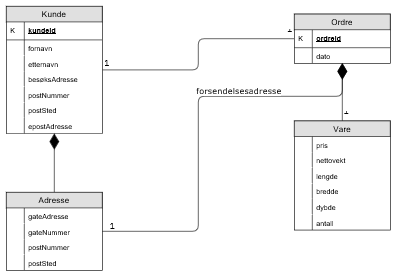
\includegraphics[scale=0.7]{fig/NettbutikkAggregatModell.png}
    \caption{Aggregatdiagram med to forskjellige entiter, modellert for den samme tjenesten fra \ref{fig1}.}
    \label{fig2}
\end{figure}

Denne figuren presenterer to forskjellige aggregatmodeller, \texttt{Kunde} og \texttt{Ordre}. \cite{sadalage2013} demonstrerer et eksempel på en aggregatorientert modell i samme forretningsdomene, med de samme to entitetene. Forbindelsen mellom disse to denoterer en én-til-mange-assosiasjon som man kjenner til fra den relasjonelle modellen, men som ikke realiseres med fremmednøkler, iallfall ikke fremmednøkler slik man er vant til dem fra MySQL og PostgreSQL. I stedet indikerer denne assosiasjonen i diagrammet at hvert kundeaggregat har en flat liste bestående av \texttt{Ordre}-nøkler som representerer alle ordrene en kunde har opprettet i netthandelen. Likeledes kan hver enkelt ordre holde på en ''fremmednøkkel'' som kun applikasjonen kan tolke, og således er det i selve applikasjonslogikken av nettbutikksystemet at ''JOIN'' blir gjort. Komposisjonselementet indikerer bruk av nøsting i aggregatet, det vil si at et Vare-objekt til enhver tid eksisterer innenfor et aggregat, nemlig \texttt{Ordre}-entiten, og aldri som et selvstendig aggregat selv. I relasjonelle ER-modeller er slik nøsting av entiteter strengt forbudt. Aggregatorienterte modeller er således \emph{denormaliserte}, det vil si at den enkelte aggregatmodell ikke oppfyller første normalform.

1NF-relasjoner består av flate tupler uten nøsting av relasjoner, eller som \cite{codd1971} definerer en unormalisert tabell: ''[a] group schema which contains a repeating group schema''. Med ''repeating group'' menes altså attributter på listeform, for eksempel en liste av strenger. Videre tillater ikke \cite{codd1971} kryssreferanse per primærnøkkel innad i en relasjon, fordi det med den egenskapen blir datamodellen rotete og vanskelig å lese for dens brukere.

En annen interessant detalj ved modellen presentert i delkapittel \ref{fig2} er at Adresse-objektet er inneholdt i både \texttt{Kunde}-aggregatmodellen og \texttt{Ordre}-aggregatmodellen. Semantikken bak er at hver ordre har en leveringsadresse som de tilknyttede varene leveres til. I praksis betyr dette at aggregater av både \texttt{Ordre} og \texttt{Kunde} lagrer potensielt samme adresseinfo, altså er adressedataobjekt lagret dobbelt opp i databasen, den er \emph{duplisert}.

Ved modellering av aggregater må man avveie mellom hvor stort hvert enkelt aggregatobjekt i en applikasjon kan bli og hvor mange forskjellige aggregatentiter applikasjonen kan ha. Alternativt kunne datamodellen i \ref{fig2} bestått av ett eneste aggregat, noe man oppnår ved å erstatte assosiasjonslinjen mellom \texttt{Kunde} og \texttt{Ordre} med en komposisjonslinje. Med to nivåer av nøstede lister av objekter innen ett aggregat, kan besvarelse av ett enkelt oppslag på én spesifikk nøkkel potensielt medføre et stort svar i retur. Responsens kan bli så stor at HTTP-responsen må deles opp i flere TCP-pakker, hvilket igjen er delt opp i mange IP-pakker som tar forskjellige ruter til den spørrende klienten.

Store, komplekse aggregat vil innvirke på spørringens nettverksforsinkelse. \cite{sadalage2013} poengterer at hvis applikasjonen alltid har bruk for å hente informasjon om ordre, samtidig som den henter informasjon om en kunde, så er det hensiktsmessig å legge ordrehistorikken til hver kunde inn under Kunde-aggregatet. Hvis applikasjonen fokuserer på kun én ordre ad gangen i dets brukervisning, så vil todelingen av aggregater som vist i \ref{fig2} være mer hensiktsmessig. Hvordan aggregater defineres er alt i alt opp til den enkelte datamodellør.

% Skriv om tre ulike aggregat - orienterte datamodeller - Segway til påfølgende delkapitler
Fowler og Sadalage omtaler tre unike datamodeller som opererer med aggregater. Nøkkel\-verdi\-modellen behandler det enkelte aggregat som en ugjennomsiktig helhet \citep{sadalage2013}. Altså går det ikke an å hente deler av aggregatet ved et nøkkeloppslag. Dokumentmodellen eksponerer aggregatet til databasen, og tillater dermed delvise spørringer.

I og med at dokumentmodellen også er skjemaløs, går det ikke an å optimalisere spørringer på hele eller deler av aggregatet. Kolonnefamilier inndeler aggregatet i grupper, noe som tillater databasen å operere på hver av disse gruppene som en egen dataenhet, liksom attributter i tuplene i den relasjonelle modellen. Selv om kolonnefamilier til dels ofrer den komplette skjemaløsheten som vi ser i nøkkel\-verdi\-modellen, har databasen nå mulighet til å nytte eksponeringen av attributter/kolonner til å optimalisere aksesseringer og oppdatere separate kolonner.

% 2.2.2
\subsection{Nøkkelverdimodellen}

Nøkkelverdi-lagre er den type NoSQL-DBMS med den enkleste aggregatorienterte datamodellen. Dens hovedkarakteristikk er at hvert aggregat som lagres må være tilknyttet én unik identifikator kalt \textbf{nøkkel}, og for å hentet det lagrede aggregatet må man vite verdien til denne nøkkelen \citep{elmasri2014}. En nøkkel er en helt unik streng som brukes av databasesystemet til å lokalisere raskt et assosisert dataobjekt (også kalt \textbf{verdi}) i en homogen klynge av databasenoder \citep{elmasri2014}.

Hvert aggregat som lagres er ugjennomsiktig, det er en stor boble av serialiserte bytes som databasesystemet ikke kan anskue. I prinsippet er nøkkel\-verdi\-modellen totalt ustrukturert, altså er det opp til selve applikasjonen hvis data lagres i nøkkelverdidatabasen å påføre dataobjektet mening og definere dets struktur \citep{elmasri2014}.

Fordelen med at aggregatet ikke synes i databasen er at applikasjonsutvikleren kan endre aggregatets struktur, også kjent som dets implisitte skjema, helt etter eget ønske. Man kan lagre hva man enn vil i et nøkkelverdilager så lenge man spesifiserer en nøkkel databasen bruker til å lete opp dataobjektet med, og følger en eventuell størrelsesbegrensning definert av databasens konfigurasjon \citep{sadalage2013}.

Spørringer skrives ikke i et domenespesifikt språk som for eksempel SQL. I stedet kaller applikasjonen på et sett funksjoner eksponert for den gjennom et applikasjonsprogrammeringsgrensesnitt (API). Dette APIet tilbyr hovedsaklig tre forskjellige spørringer: Lesespørring (\texttt{GET}), skrivespørring (\texttt{PUT}) og slettespørring (\texttt{DELETE}). Både oppdateringer og opprettelser av dataverdier gjøres med én og samme kommando, PUT. Enkelte nøkkelverdidatabaser kan supplere med flere funksjoner til for eksempel administrative behov. Hver enkelt spørring behandler \underline{ett helhetlig aggregat av gangen}. En lesespørring på en nøkkel henter ut hele aggregatobjektet assosiert med nøkkelen. En skrivespørring som oppdaterer et dataobjekt skriver over eksisterende data assosiert med objektets nøkkel fullstendig.

Moderne, populære NoSQL-systemer avviker noe fra dette prinsippet som skiller nøkkel\-verdi\-modellen fra dokumentmodellen. I dokumentlagre går det an å definere et ID-felt, en primærnøkkel, brukt til å gjøre ID-oppslag på samme vis som i et nøkkelverdilager. Riak KV tillater applikasjonsutvikleren å legge inn metadata direkte inn i det lagrede aggregatobjektet slik at deler av aggregatet indekseres, og det samme systemet implementerer også en form for assosiasjon mellom aggregater. Videre har Riak også en søkefunksjon som kan brukes på JSON-serialiserte aggregater \citep{sadalage2013}. Redis, et annet nøkkelverdisystem, støtter lagring på og oppslag av aggregatobjekter som ikke likner på tradisjonelle JSON-objekter, men objekter i form av lister, hashede verdier og mengder.

I kraft av databasens egenskap i å støtte kun én eneste indeks, nemlig oppslagsnøkkelen til dataobjektene, er nøkkel\-verdi\-modellen forenlig med systemkrav om at datavolumet som lagres skal jevnfordeles utover en klynge av uavhengig opererende databasenoder. Å ta høyde for aggregateksponering til datalageret, direktereferanser til andre aggregat, og delvis indeksering på aggregatet, gjør oppfyllelse horisontal skalerbarhet i databasen vanskeligere. Videre er kontroll av transaksjonskonsistens (også kjent som ''Consistency'' i ACID-forkortelsen) en jobb som i utgangspunktet ''outsources'' til applikasjonen, fordi nøkkelverdi-lageret er prinsipielt uvitende om den bakenforliggende semantikken til det enkelte dataobjekt.

% 2.2.3
\subsection{Dokumentmodellen}

I motsetning til nøkkelverdilagre er det enkelte aggregatobjekt sin datastruktur synlig for dokumentlagre, som også kan utføre både lesespørringer og oppdateringsspørringer på spesifikke feltvariable innen de lagrede aggregater, altså bare hente ut distinkte deler av dokumenter. Dokumentlageret kan lese av disse ''selvbeskrivende dataene'' \citep{sadalage2013, elmasri2014} som finnes i aggregatobjektene, og derfor er slike delvise spørringer mulig. De enkelte attributter innen aggregater som er interessant for en applikasjon kan også indekseres av databasen på samme måte som relasjonsdatabaser er i stand til å indeksere enkeltattributter i relasjoner. Samtidig fører dokumentlageret begrensninger på hvordan strukturen til det lagrede aggregatet kan se ut, gjennom definisjoner av tillatte datatyper og objektstrukturer \citep{sadalage2013}. På tross av at dokumentdatabasen kan anskue aggregatets struktur, opererer hver enkelt spørring på ett enkelt, helhetlig dokument av gangen.

Dokumentlagere inndeler vanligvis data i samlinger (eng. ''collections'') av dokumenter (eng. ''documents''). De enkelte dokumenter er aggregatobjekter utformet i et semistrukturert format, som XML eller JSON. Dokumenter lagret innen samme dokumentsamling tillates å ha forskjellige definerte eller udefinerte verdier for enkelte variable. Denne fleksible egenskapen er ikke å finne i den relasjonelle modellen.

Spesifikt i MongoDB lagres dokumenter i BSON, et binært format som er en utvidelse av JSON-standarden med noen ekstra datatyper, optimalisert for lagring på disk. For å opprette en ny dokumentsamling har MongoDB metoden \texttt{createCollection}, som tar inn samlingens navn og en mengde innstillinger som bestemmer begrensninger for samlingen, som for eksempel det totale datavolumet og det maksimale antallet dokumenter som samlingen kan holde på. Hvert dokument har et automatisk generert felt som MongoDB bruker som primærnøkkel, med mindre applikasjonsutvikleren definerer en slik indeks selv \citep{elmasri2014}.

Dokumentsamlinger er ikke bundet til et skjema slik som relasjonelle databaser. Strukturen til aggregatet/dokumentet defineres av applikasjonens utviklere, og velges utifra applikasjonens krav til datamodellen, i stedet for at applikasjonens logikk tilpasser seg en rigid, todimensjonal struktur slik vi ser i relasjoner. Følgelig blir det umulig for databasesystemet å optimalisere spørringer med basis i aggregatstrukturen, fordi den er ikke gitt før innsettingsspørringer tikker inn (i kontekst av Mongo via \texttt{insert} - funksjonen).

% 2.2.4
\subsection{Kolonnefamiliemodellen}

Googles BigTable er et databasesystem som har inspirert mange senere NoSQL-systemer, akkurat som Dynamo. BigTable er en ofte brukt lagringsteknologi hos Googles applikasjoner, deriblant Gmail \citep{elmasri2014}. Apache HBase er et kolonnefamilielager tilgjengelig i åpen kildekode\footnote{Tilgjengelig på følgende GitHub-repositorium: \url{https://github.com/apache/hbase}} som implementerer de sentrale teknikkene inneholdt i BigTable.

Kolonnefamilielagre kan beskrives av \cite{elmasri2014} som ordnede, flerdimensjonale, distribuerte ordlister, hvorav nøkkelverdilagre som Redis kan ansees å være enkeltdimensjonale, distribuerte ordlister. Den enkelte aggregat-nøkkel i et kolonnefamilielager består av flere distinkte komponenter, vanligvis et navn på samlingen av aggregater, en nøkkel som identifiserer selve aggregatet (''row key''), aggregatet i seg selv som også refereres til som en ''kolonne'' og et tidsstempel \citep{elmasri2014}.

\newpage

% Figur 3
\begin{figure}[!ht]
    \centering
    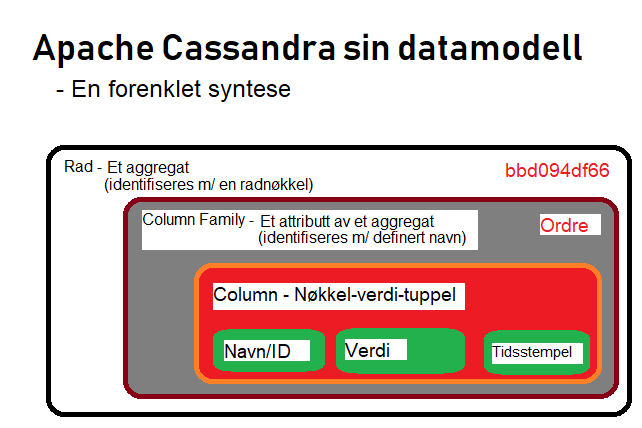
\includegraphics[scale=0.7]{fig/kolonneorientert.png}
    \caption{Metamodell som viser forholdene mellom dataenheter i Cassandras logiske datamodell.}
    \label{fig3}
\end{figure}

I et kolonnefamilelager er hvert enkelt aggregat identifisert av en todimensjonal nøkkel: Den ene komponenten er en radnøkkel og den andre er navnet på en kolonnefamile underordnet ''raden'', som i Cassandra er en samling aggregater (se \ref{fig3}). En kolonnefamilie er en samling nøkkel-verdi-tupler, ikke ulikt en tuppel og dens attributter i den relasjonelle datamodellen.

I eksempelet i \ref{fig2} med aggregatmodellen måtte man i de øvrige to datamodellene velge mellom å ha én entitet, Kunde med \emph{n} Ordre underordnet, eller to altså at lesing av kundedata innebærer raskere lesing på disk, men innhenting av alle ordre må gjøres med \emph{n} enkeltoppslag når listen av ordreID-er i kundens ordreliste er av størrelse \emph{n}. I et kolonnefamilielager kan man i prinisppet få i pose og sekk ved å definere hvert aggregat til å representere en kunde og la samlingen av \texttt{Ordre}-entiteter underordnes som en kolonnefamilie i tillegg til å definere en annen kolonnefamilie, Profil, som inneholder kundens personlige data og leveringsadresse. Hvis applikasjonen nå er interresert i en kundes profildata, slipper den å hente alle dens ordre i tillegg.


% Teorien som legger til grunn for Project Voldemort
\section{Amazon Dynamo}

Her rettes fokuset mot en berømt artikkel hvis primære fokus var å besvare Amazon sitt problem med skalering av skriveoperasjoner i et kommersielt netthandelsystem som betjener flere hundre tusen forbrukere verden over. Den hypotetiske systemarkitekturen artikkelen beskriver, Dynamo, er stamfar til mange populære NoSQL-databasesystemer lansert som åpen kildekode, deriblant Apache Cassandra, Basho Riak, Amazons DynamoDB og Linkedins Project Voldemort. Drivkraften bak designet av dette likemannssystemet er den samme som den bak vårt ønske om å kunne migrere data levende i det distribuerte produksjonsmiljøet: Høyere tilgjengelighet for interaksjon mellom brukernes klientapplikasjoner og deres databasetjenere. Derfor er en god forståelse av problemstillingene og utfordringene Dynamo løser, samt hvordan løsningene kan implementeres, relevant for oppgavens problemstilling.

\subsection{Bakgrunn for artikkelens arbeid}

% Introduksjon/Abstract
\cite{decandia2007} presenterer arkitekturen til Dynamo, et høytilgjengelig, distribuert nøkkel-verdi-lager som ved nettverkspartisjoner ofrer replikakonsistens til fordel for å være mottakelig for lese - og skriveforespørsler fra diverse mikrotjenester som lever i Amazons applikasjoner. I kjernen av problemet denne distribuerte databasearkitekturen forsøker å løse ligger et sterkt krav til at enhver kunde av Amazons netthandel alltid skal kunne legge artikler i handlekurven. Handlekurven i nettbutikken, så vel som hver eneste artikkel i nettbutikken skal til enhver tid kunne interageres med. Ethvert avbrudd i denne tjenesten kan og vil medføre monetære tap enten direkte i form av utsatte handler og indirekte i form av økende mistro hos forbrukerne. Amazon.com er samlet sett en gigantisk, distribuert netthandelapplikasjon bestående av mange tusen nettverkskomponenter og uavhengige tjenere spredt utover mange datasentre. I denne infrastrukturen er feil som oppstår i enkeltkomponenter normen, ikke unntaket.

Amazon.com er en av verdens største ekommersplattformer. Den består av flere tusen uavhengige tjenerkomponenter lokalisert i flere datasentre verden over, og betjener flere titalls millioner kunder samtidig ved julehøytider når besøkstrafikken er på sitt høyeste \citep{pepitone2010}. Et knippe av disse tjenestene er illustrert som testimonale på økosystemets diversitet i figuren ''Figure 1'' i \citep{decandia2007}. Hvis én enkelt komponent i den avanserte tjenestearkitekturen netthandelen avhenger av for å være oppegående påkrever vedlikeholdsarbeid går det ikke an å ta ned hele nettbutikken fullstendig for så mye som en time uten å tape en uutholdelig mengde millioner dollar i urealiserte inntekter. Derfor stilles svært høye ytelses - og pålitelighetskrav til denne ekommersplattformen. I tillegg må dette komplekse systemet kunne skaleres horisontalt inkrementelt, altså at det distribuerte systemet kan utvides med én lagringsnode av gangen med minimal påvirkning på dets tjenesteytelsesevne.

I et stort, distribuert system vil fatale tjenerfeil, det vil si feilscnarier der en enkelt tjener følgelig blir utilgjengelig for dets brukere, inntreffe jevnlig, og med høy frekvens. Bevis: Hvis variabelen \(N\) denoterer et stort antall tjenere i et distribuert system, og sannsynligheten for at én tjener lider en fatal tjenerfeil i løpet av ett døgn estimeres til \(p\), så er sannsynligheten for at minst én tjener i klyngen blir utilgjengelig gitt ved \(1-(1-p)^s\). Et konkret eksempel: \(p=0.05, s=50 => 1-(1-p)^s=0.9231\). I en mellomstor klynge med 50 tjenere og hver feiler med en sannsynlighet på fem prosent i løpe av ett døgn, så er sannsynligheten for at samtlige tjenere er oppegående i løpet av ett helt døgn under åtte prosent. For at så lite datavolum skal være utilgjengelig til enhver tid i et distribuert databasesystem må det fordele datalasten jevnt utover alle tjenerne i tillegg til å bestå av mange tjenere.

Helt siden deres framvekst på 80 - tallet har applikasjonsdata i større produksjonsmiljø blitt lagret av relasjonelle databasystemer. \cite{decandia2007} anser imdlertid transaksjonsbasert lagring som en suboptimal og ineffektiv løsning for sitt eget produksjonsmiljø, av hovedsaklig to årsaker:

\begin{description}
  \item [Horisontal skalerbarhet] Som vist i det tidligere nevnte hypotetiske systemet Hush \citep{george2011} er tradisjonelle relasjonsdatabaser lite fleksible når det kommer til datareplikering i distribuerte databaser. \cite{decandia2007} bemerker også at det er vanskelig å skalere ut og partisjonere data jevnt utover lagringsnodene i distribuerte, relasjonelle databasesystemer, til tross for at de mest avanserte relasjonelle DBMSene støtter noen former for klyngeoperasjoner.
  \item [Unødvendige DBMS-funksjoner] Tjenestearkitekturen til Amazon har behov for en svært begrenset mengde funksjoner fra dets datalager, og sjelden behøves det at databasen skal kunne utføre avanserte oppgaver som triggere og lagrede prosedyrer, eller kjøre komplekse spørringer aggregeringsoperasjon som summering og gjennomsnitt på enkeltverdier på enkeltattributter over flere dataobjekter. Flesteparten av de enkeltstående tjenestene som eksempelvis handterer bestselgerlister, handlevogner, kundepreferanser, salgsstatistikk, og innloggingsdata, både spør etter og persisterer dataobjekter utelukkende på enkeltnøkler, altså er de korresponderende abstrakte relasjonsmodellene for hver av disse uavhengige tjenestene assosiasjonsløse, det vil si at de kan modelleres som én enkeltstående, kompleks entitet, med nøsting av objekter og lister.
\end{description}

Følgelig går Dynamo inn for en enkel spørringsmodell: Ethvert dataobjekt identifiseres med en unik (hash)nøkkel. Alle skrive - og leseoperasjoner i lagringssystemet gjøres gjennom oppslag på en slik ID. Samtlige spørringer gjøres på ett enkelt dataobjekt ad gangen slik at det ikke er behov for å innføre støtte assosiasjoner mellom ''tuplene'' i datamodellen.  % Skriv om spørrings-APIet til Dynamo

Dynamo sitt systemdesign ble primært laget for å kunne tekkes Amazons storskala - produksjonsmiljø med flere titalls millioner samtidig påloggede forbrukere. Det distribuerte lagringssystemet som realiserer Dynamos arkitektur er designet både for tilgjengelighet og skalerbarhet. Førstnevnte kvalitetsattributt realiseres gjennom planlegging for feilsituasjoner, og motvirkelse av effektene en diverse typer feil som kan oppstå i for eksempel nodens maskinvare eller dens kjørende programvareprosess kan ha. Sistnevnte oppfylles ved å implementere en lastbalanseringsalgoritme som fordeler ansvaret for lagring av de enkelte dataobjektene utover nodene i lagringssystemet, og som kan omfordele data skulle én av lagringsnodene svikte og bli utilgjengelig.

Utviklerne bak Dynamo valgte av hensyn til tilgjengelighetskravene å gjøre replikering av dataobjekter asynkront, derav kan ikke det samme skrivekonsistensnivå som vi finner hos relasjonelle databasesystem oppfylles. Årsaken til dette tilfellet er at datalagret hverken kan eller vil kontrollere hvorvidt hver enkelt spørring mottar eller opererer på dataobjektets nyeste utgave, altså tillater databasen lesing av foreldete data. Hva angår ACID - egenskapene fokuserer Dynamo på å opprettholde atomisiteten til spørreoperasjonene, på grunn av kravene \cite{decandia2007} stiller til spørringsmodellen. Altså lagrer Dynamo aggregatobjekter som innehar hele den persisterte tilstanden som applikasjonene til Amazon opererer på i primærminne. Av hensyn på skrive-tilgjengeligheten isoleres ikke spørringsoperasjonene, hvilket betyr at systemet tillater at skriveoperasjoner mistes ifølge Last Write Wins - prinsippet. Av økonomiske hensyn er det også viktig at Dynamo, det distribuerte nøkkelverdilageret, kan kjøre på en infrastruktur bestående av billige datamaskiner, hvilket betyr få prosessorkjerner og begrenset datavolum både i primærminnet (RAM) og sekundærminne (platelager).

Artikkelens vitenskaplige bidrag er en vurdering av hvordan ulike algoritmer og teknikker kan kombineres til å implementere et høytilgjengelig nøkkelverdilager. Den viser at en database som ikke garanterer et strengt konsistensnivå trygt kan brukes i et produksjonsmiljø der frekvensen av innkommende spørringer er høy. Artikkelen viser også hvordan et slikt nøkkelverdilager kan konfigureres til å oppfylle strenge ytelseskrav i høytraffikerte produksjonsmiljø \citep{decandia2007}.

\subsection{Om Dynamos arkitektur og Amazons implementasjon} \label{dynark}

Designet til et distribuert nøkkelverdlager som opererer i et stort produksjonsmiljø slik som Dynamo må nødvendigvis være ganske komplekst, fordi det er mange problemer som må løses av dette designet som en monolittisk databasearkitektur ikke har. For å tekkes strenge krav til tilgjengelighet må systemet ha gode løsninger til lastbalansering av data, datareplikering, dataobjektversjonering, og feilhandtering.

Dynamos logiske ring av noder som lagrer data er et likemannsnettverk. Et likemannsnettverk er en distribuert programvarearkitektur der alle noder utfører de samme arbeidsoppgavene. I et likemannsnettverk har hver enkelt node kjennskap til et visst antall andre noder i nettverket, gjerne referert til som ''naboer'', ved hjelp av en routingtabell, som er en oppslagsliste hver enkelt node kan bruke til å finne ut hvilken node en forespørsel bør videresendes ved behov.

I tråd med artikkelens observasjon vedrørende Amazon-applikasjonenes begrensede behov for spørringsfunksjonalitet i databasen de kontakter har Dynamo-implementasjonen beskrevet av \cite{decandia2007} definert et spinkelt spørrings - API bestående av to funksjoner: \texttt{get(\emph{key})} og \texttt{put(\emph{key, context, object})}. \texttt{get} - funksjonen er for lesespørringer. Hver lesespørring er et oppslag på en nøkkel, \emph{key}, som er tilknyttet et dataobjekt på binær form. Når \texttt{get} kalles, vil databasenoden som mottok spørringen, i artikkelen referert til som \underline{koordiantoren}, først identifisere nodene som lagrer replikaene av det ønskede dataobjektet og kontakter alle nodene som holder på disse replikerte objektene. Det aggregatet med den nyeste versjonen returneres til applikasjonsklienten. Spørringen kan også returnere en liste av objekter hvis dataversjoner divergerer, i tillegg til tilhørende metadata - da må de divergerende aggregatene flettes sammen, og en ny versjon må deretter persisteres. Amazons implementasjon av Dynamo anskuer både nøkkelen og dataobjektet som en ugjennomsiktig streng av biter.

\cite{decandia2007} sin implementasjon av Dynamo bruker Last-Write-Wins-strategien som konfliktresolusjonsalgoritme, hvilket er en lettvint løsning: Ved fletting lagrer databasenoden simpelthen den oppdateringen på det vedkommende dataobjekt som har det seneste tidsstemplet eller har høyest vektor-klokkeverdi, således vil en skriveoperasjon gå tapt for programvaresystemet Dynamo lagrer data for. Per nøkkelverdidatamodellen sin natur er det urimelig å forvente at det distribuerte datalageret har noen form for semantisk kjennskap til dataobjektene den tar hand om, da de for databasenodene bare er lemfeldige samlinger av binære tall. Derfor kan appliaksjonsutviklere implementere sine egne konfliktresolusjonsalgoritmer som påkalles hvis samtidige skriveoperasjoner gjør at to replikaer av et aggregat divergerer versjonshistorisk sett. For Amazon sine hovedsaklige bruksområder for Dynamo er ikke tapte skrivinger et problem, med unntak av handlevognsapplikasjonen kundene bruker i nettbutikken. Loggdata er ikke like kritisk som handledata, så der kan LWW-fletting trygt brukes.

\texttt{put} - funksjonen brukes til både å opprette og oppdatere lagrede dataobjekter assosiert og slått opp på nøkler. Når \texttt{put} kalles, blir først nodene som er ansvarlige for dataobjektet identifisert og kontaktet på samme måte som i \texttt{get}. I tillegg til aggregatets nøkkel, \emph{key}, har \texttt{put} to andre argumenter, \emph{context} og \emph{object}. \emph{context} - variabelen representerer metadata om dataobjektet som lagres, deriblant verdiene i dets vektorklokke. Informasjonen i \emph{context} - variabelen brukes også til å sammenliknes med tilsvarende lagret metadata i databasen for å validere dataobjektet som sendes inn i som argument i \texttt{put} - kallet.

For å identifisere hvilken node i likemannsnettverket som skal ha ansvar for oppslaget på en nøkkel \emph{k} blir den hashet med MD5-algoritmen som returnerer en 128-bit streng \emph{h} hvis verdi faller imellom to andre IDer som hver identifiserer én separat databasenode i hashringen. Den databasenoden hvis ID er nærmest, men lavere enn \emph{h} i binærtallsystemet er den noden som får ansvar for å levere dataobjektet med nøkkel \emph{k} ved spørringer etter denne nøkkelen.

For konsistenskontroll bruker Dynamo en egen protokoll inspirert av quorumreplikering \footnote{Begrepet \emph{quorum} er latin og betyr ''beslutningsdyktig antall''} for å replikere dataobjekter. Quorum-replikering er en datareplikeringstrategi for distribuerte datalagre som er justerbar. Et quorum er en mengde noder som tilordnes ansvaret for en spørring, til vanlig av en valgt koordinator. \cite{bailis2014} viser gjennom simulasjoner med en probalistisk sannsynlighetsmodell og evaluering av loggdata innsamlet i store, kommersielle produksjonsmiljø at quorumreplikerte databasesystemer lar databaseadministratorer i prakis stille på konsistensnivået til samtidige spørringer ved å konfigure en tuppel bestående av følgende tre tall som indikerer antallet replikeringsoperasjoner for hver innkommende forespørsel:

\begin{itemize}
  \item R - quorumstørrelse for leseoperasjon
  \item W - quorumstørrelse for skriveoperasjon
  \item N - Antall replikerte dataelementer for én enkelt nøkkel
\end{itemize}

I kontekst av Dynamo er dens replikeringsalgoritme ekvivalent med et strikt quorumsystem hvis R, W og N er definert slik at begge av følgende betingselser er oppfylt:

\begin{itemize}
  \item \(W > N/2\), altså at spørringskoordinatoren avventer bekreftelser på at over halvparten av de N replikaene fullbyrdet spørringen
  \item \(R + W > N\), altså at mengden replikaer av et aggregat spørringskoordinatoren venter på før ett av disse returneres til databaseklienten overlapper med mengden bekreftelsesmeldinger fra en skrivespørring spørringskoordinatoren venter på før den returner en bekreftelsesmelding til klienten
\end{itemize}

I et strikt quromsystem oppfylles sterk replikakonsistens, enhver lesespørring på et dataobjekt får med seg dens siste oppdatering/PUT som er skrevet til disk nettopp fordi minst én node er med både i dataobjektets skrivequorum og dets lesequorum. Det må påpekes at strikte quorumsystem venter på at samtlige noder i ethvert quorum returner svar på forespørselen fra spørringskoordinatoren, det vil si at strikte quorumsystem øker nettverksforsinkelsen til hver enkelt spørring for å sikre sterk replikakonsistens, fordi koordiantoren må nødvendigvis vente på den noden i quorumet der spørringen har høyest forsinkelse i nettverket (her antas det at nettverks-I/O er langt mer tidkrevende enn I/O-operasjoner på et platelager lokalt).

Quorum-replikeringsstrategien til Dynamo avviker et ordinært quorumsystem på to fronter. For det første: Hvis Dynamo hadde brukt et strikt quorumsystem for datareplikering ville enkelte dataobjekter ha blitt utilgjengelige for databaseklientene hvis nettverkspartisjoner i ringen oppstår, eller hvis de simpleste feilscenarier der bare én enkelt node rammes inntreffer. I tillegg ville skrivespørringer være i langt mindre grad holdbare (''durable'') på disk \citep{decandia2007}. For det andre er Dynamos quromprotokoll ''sløv'', det vil si at en spørringskoordinator oppnevner ikke en bestemt mengder noder som alle \textbf{må} fullføre spørringen for at resultat kan sendes tilbake til databaseklienten som gjorde spørringskallet. Fordelen med denne sløvheten, eller skal vi heller si ''fleksibiliten'', er at risikoen for at en spørring ikke blir besvart på grunn av at én enkelt node er utilgjengelig minimaliseres. For en høytilgjengelig nettbutikk so Amazon.com er nettverksforsinkelse et mye større problem enn synkronisering av replikaer, derfor konfigureres quorumet gjerne slik at \(R + W < N\), for eksempel \(R = 1, W =1, N = 3\).

For øvrig kan Dynamo sine kjerneegenskaper oppramses som følger:

\begin{description}
  \item [Konsistent hashing] Lastbalanseringsalgoritmen Dynamo bruker for å partisjonere data utover ringen av databasenoder, hvilket er formen til den strukturen til likemannsnettverket, av databasenoder. Både data og nodeidentifikatorer hashes inn i ringen. En node, det vil si en tjenerprosess i ringen, lagrer eller holder rede på dataobjekter som har blitt hashet til forgjengernoden i ringen, således realiseres lastbalansering i et likemannsnettverk bestående av mange tjenere på en ryddig måte. Den konsistente hashalgoritmen oppfyller kravet om inkrementell skalerbarhet.
  \item [Vektorklokker] Versjoneringsteknikk brukt til å holde styr på oppdateringshistorikken til et dataobjekt. Hver databasenode som oppdaterer et bestemt aggregat skriver et stykke metadata, en vektor på formen (\texttt{nodeNo}, \texttt{seqNo}), der førstnevnte representerer den enkelte noden som skriver dataobjektet, mens den andre variabelen er et versjonsnummer (eventuelt et tidsstempel) som øker monotont for hver gang objektet skrives til disk. Ved å lese av denne vektoren kan man utlede endringshistorikken til hvert enkelt dataobjekt og se kausaliteten mellom forskjellige \underline{versjoner} av det, altså hvilke skrivinger som er fundert på tidligere skrivinger. Hvis to samtidige oppdateringer medfører to divergerende versjoner kan versjonshistorikken brukes til å identifisere ''synderne'' som utførte de uavhengige oppdateringene og deretter finne ut hvilke datahverdier innad i de divergerende objektene som skal beholdes under fletteprosessen, som utføres i klientdelen av databasearkitekturen.
  \item [Slurvete quorum (eng. Sloppy quorum)] Lese - og skriveoperasjoner utføres på de første N ''friske'' databasenodene ifølge en preferanseliste konfigurert globalt i systemet. Noder som ikke responderer på forespørsler, dvs ''syke'' noder, hoppes over. Denne midlertidige økningen av medlemmer i quorumet kalles også for antientropi.
  \item [Antydet avlevering (eng. Hinted handoff)] Teknikk for hurtig handtering av innkommende skrivinger addressert til en utilgjengelig node. Når den slurvete quorumalgoritmen finner at én av addressentene i skrivequorumet er (midlertidig) utilgjengelig, så blir skrivequorumet midlertidig utvidet med en ekstra ''oppassernode'', som lagrer dataobjektet helt til den frafalne noden er tilbake i ringen. Når oppassernoden mottar nyheter (via sladderprotokollen) om at noden som dataene opprinnelig tilhører lever igjen, blir disse avlevert til sitt opprinnelige tiltenkte lager fra oppassernode.
  \item [Merkle - trær] Et Merkle-tre er et hashtre der hver enkelt løvnode holder på en hashet verdi. Foreldrenodens tilstandsverdi tilsvarer den kumulative hashverdien av dens barn. Rekursivt sett vil dette si at rotnoden holder på den sammenlagte verdien for alle løvnodene i treet. Hvert enkelt nivå i treet er følgelig sammenliknbart med korresponderende nivå i liknende tre.
  \item [Antientropi] Mens slurvete quroumoperasjoner og antydete avleveringer kan brukes til å respondere på midlertidige fravær av noder, som kan forårsakes av at et unntak kastes i selve programvareprosessen til noden, benyttes Merkle - trær til å rebalansere datalasten i likemannsnettverket etter at en databasenode legges til eller blir permanent utilgjengelig. Merkle-trær er således en viktig datastruktur for å realisere antientropi-protokollen til Dynamo. Merkle-trær brukes til å synkronisere utdaterte replikaer uten å sende én enkelt melding per oppdaterte replika av hvert eneste lagrede dataobjekt. Istedet kan hver enkelt par av noder utveksle en hash-verdi som representerer den samlede hashverdien for deres respektive nøkkelrom. Når en node legges til eller forsvinner fra ringen, må nøkkelintervallene som nodene er ansvarlige for å lagre omfordeles for å fordele datalasten jevnt. Hvis ringen har høy ''churn'' - rate, det vil si at noder svært ofte kommer og går ut av ringen eller at fatale eksekveringsfeil oppstår abnormalt ofte hos nodene, vil nøkkelintervallene bli rekalkulert svært ofte, noe som hemmer ytelsen til systemet.
  \item [Sladder-basert medlemskapsprotokoll (eng. ''Gossip-based membership protocol'')] ''Gosipping'', eller ''sladder'' på godt norsk, er en masterløs, skalerbar medlemskapsprotokoll der hver enkelt node jevnlig kontakter en tilfeldig valgt nabo (''peer'') og utveksler og oppdaterer egne registrerte medlemsdata om ringen. \cite{decandia2007} registrerer også at denne ''explicit node join'' - prosessen gjør at noder blir oppmerksomme både på nye noder og nylig utilgjengelige noder hvilket gjør en separat distribuert feildetektor overflødig. På grunn av protokollens asynkrone natur (hver enkelt medlemskapsendring i ringen medfører ikke en direkte oppdatering hos alle nodene samtidig utstedt fra en sentral medlemskoordinator) er medlemslistene svakt konsistente. Hensikten med en slik medlemsprotokoll er både å holde styr på hvilke databasenoder som fortsatt er del av Dynamo-ringen og å detektere at en node er utilgjengelig, dvs at den er utsatt for feil, slik at systemet kan midlertidig persistere replikaer offeret for feilen hadde styr på hos noen andre noder med antydet avlevering.
  \item [Lesereparasjon (eng. ''Read repair'')] I Amazons implementasjon venter den enkelte databasenode på respons fra spørringskordinatoren etter å ha returnert et dataobjekt til den. Hvis spørringskoordinatoren under lesespørringen mottok dataobjekter som ikke er av den nyeste versjonen, dvs at enkelte aggregatreplikaer er utdaterte/''stale'' \citep{decandia2007}, kan den sende tilbake skriveforespørsler med den nyeste versjonen den til de respektive noder som returnerte de utdaterte dataobjektene. Prosessen bærer navnet ''lesereparasjon'' fordi replikaer som ikke har fått med den seg den nyeste dataversjonen blir opportunistisk reparert av spørringskoordinatoren. Denne prosessen kjøres ad-hoc og er ikke effektiv når det kommer til å synkronisere replikaer ved endringer i medlemsmassen til Dynamo-ringen.
\end{description}

Denne teknologiske syntesen, tildels inspirert av distribuerte hashtabeller og quorumsystemer medfører i sum et høytilgjengelig, feilrobust, lastbalansert nøkkelverdilager hvis kvalitative lagringsegenskaper kan fininstilles ved å konfigurere quorumvektoren (R, W, N). Mange av disse teknikkene er, som vi skal se i neste delkapittel, også realisert i Project Voldemort.

% Om Project Voldemort
\section{Project Voldemort}

Project Voldemort er et distribuert nøkkelverdilager inspirert av Amazons nøkkelverdilager Dynamo, hvis arkitektur presenteres av \cite{decandia2007}. Dette systemet replikerer og partisjonerer sine data automatisk. Forfatterne og vedlikeholderne \footnote{Kildekoden til Project Voldemort er lisensiert under Apache 2.0 - lisensen, og er tilgjengelig på følgende GitHub-repositorium: \url{http://github.com/voldemort/voldemort/tree/master}} av kildekoden refererer til Voldemort som en stor distribuert, persistent, feiltolerant hash-tabell \citep{kreps2009}. Hver enkelt node i det kjørende databasesystemet holder en delmengde av den totale datamengden som handteres. Flere komponenter i dette systemet, deriblant databasemotoren, plasseringsstrategien for data-tupler, og serialiseringsmetoden, er valgfrie for den enkelte programmerer. Blant annet kan man bruke lagringskomponenter som InnoDB, RocksDB (som benytter LSM-trær), Berkeley DB, eventuelt kan man lagre tupler i primærminnet. I tillegg er også nivået på konsistens av skriveoperasjoner justerbart. Prosessperspektivet til arkitekturen er master-fri, det vil si at i det distribuerte datalageret holdes det ikke valg av spørringskoordinator blant nodene. Derfor opererer de som et likemannsnettverk. Feil som oppstår ved spørringseksekvering behandles transparent.

\subsection{Støttede operasjoner}
Nøkkelverdilagre tilbyr tradisjonelt sett et svært enkelt spørregrensesnitt til applikasjoner som bygger sine datamodeller med dem. Og Voldemort er overhodet ikke annerledes i den forstand. Applikasjonprogrammerings-grensesnittet til Voldemort definerer hovedsakelig tre funksjonelle endepunkter: \texttt{get} (leseoperasjoner), \texttt{put} (skriveoperasjoner, både til opprettelse og oppdatering av tupler), og \texttt{delete} (sletteoperasjoner). I tillegg til disse tre operasjonene som er karakteriske for de fleste nøkkelverdilagre definerer Voldemorts klient – API endepunktene \texttt{getAll}, som er en leseoperasjon på multiple nøkler, og versjonerte utgaver av \texttt{get} og \texttt{put} som til forskjell fra de ordinære funksjonene med samme navn tar inn et versjonsobjekt som input til funksjonen i tillegg til en nøkkel og en verdi, slik at tjeneren slipper å gjøre et oppslag for å finne den nyeste versjonen til det angitte objektet først. Hvis versjonen av objektet hvis nøkkel er spesifisert i funksjonskallet ikke er den nyeste vil klientprogrammet kaste et unntak, kalt \texttt{ObsoleteVersionException}, og brukeren får ingenting returnert. Som tidligere nevnt i den generelle diskusjonen om nøkkelverdilagre anser en databasenode hos Voldemort både nøkkel og det assosierte dataobjekt som en tilfeldig sekvens of bytes. % bryt-opp

% Som et interressant apropos eksponerer \emph{StoreClient} - grensesnittet til Voldemorts kildekode en tredje variant av de to spørringene.  \texttt{get} og \texttt{put}: En variasjon som tar inn en transformsfunksjon som kjøres av databasenodene som mottar disse spørringene før (put) eller etter (get) de oppdater eller henter sitt eget datareplika. Disse funksjonene er nyttige for den som vil implementer en Voldemort-databaseklient i Java som kan migrere data levende hvis det implisitte skjemaet til den ovenstående webapplikasjonen blir endret. % ??

\subsection{Voldemorts egenskaper sammenliknet med RDBMS}
I forhold til relasjonelle databasehåndteringssystemer er Voldemort vesentlig bedre egnet til å innføre replikering av data, da ytelsen til både leseoperasjoner og skriveoperasjoner lar seg skalere horisontalt. Det vil si at hvis en ny node legges til det distribuerte miljøet, også benevnt i litteraturen som ''databaseinstansen'' \citep{sadalage2013}, så vil det ha ingen eller neglisjerbar påvirkning på ytelsen. 

Et relasjonelt DBMS har den fordel over Voldemort at dets innebygde samtidighetshånd\-tering, som utføres ved hjelp av transaksjonsmønsteret, er strengere og derfor mer pålitelig enn Voldemort. Voldemort fokuserer heller på å holde orden på endringshistorikken til hver enkelt tuppel som lagres på den enkelte node i det distribuerte lageret. Ved hjelp av versjonering kan kopier, eller replikaer, av tupler hvis dataverdier er divergerende, rettes opp gjennom en flettingsprosess.

Moderne webapplikasjonssystemer består gjerne av forskjellige, adskilte tjenester eller applikasjonsgrensesnitt, hver av disse kan i sin tur distribuere egne data over opptil flere datasentre rundt om i verden. Slike webapplikasjoner kan ikke ta seg tid til å vente på JOIN - operasjoner mellom to entiteter eller tabeller som potensielt ligger på hver sin MySQL - tjener på hver sin datamaskin i hvert sitt datasenter på to vidt forskjellige lokasjoner på kloden. Én framgangsmåte på å skalere en relasjonell datamodell til å møte behovene til flere tusen forespørsler samtidig, er å introdusere et hurtiglager-nivå i systemarkitekturen ved hjelp av et distribuert, minnebasert cachesystem som MemCache eller Redis. Dette hurtiglageret avlaster databasen for leseoperasjoner, som vil utgjøre en flaskehals for den samlede ytelsen til den distribuerte applikasjonen. Dessverre vil ikke denne løsningen skalere for skriveoperasjoner og JOIN - operasjoner så lenge logisk konsistens for skrivinger er et krav. Voldemorts løsning, hvis tekniske detaljer vil bli diskutert i neste delkapittel, er å lempe på disse konsistenskravene.

Relasjonelle databasesystemer realiserer de assosiasjoner som er spesifisert mellom entitetene i datamodellen til applikasjonens arkitektur. Relasjonelle databasesystemer oppfyller samtidig fire egenskaper for skriveoperasjoner som gjøres i systemet gjennom transaksjonsmønsteret. Atomisitet, en garanti på at hver enkelt transaksjon enten utføres fullt og helt eller avbrytes; Konsistens: for hver enkelt utførte transaksjon etterlates databasen i en konsistent tilstand; Isolasjon: Hver enkelt transaksjon kjøres uavhengig av hvilke andre transaksjoner som kjøres samtidig; Holdbarhet: Data som er persistert gjennom transaksjoner i systemet, vil ikke endres eller forsvinne med mindre påfølgende transaksjoner gjør det. Hver enkelt PUT-operasjon i Voldemort er atomisk så lenge den opererer på et og samme aggregat i datamodellen, det vil si den komplekse objektverdien som aksesseres med nøkkelen.

Transaksjoner gjør skriveoperasjoner i relasjonelle databaser lineariserbare, som er det strengeste konsistensnivået skriveoperasjoner kan ligge på i databasesystem, ved å tvinge skriveoperasjonen til å vente hvis den prøver å endre rader eller tabeller som allerede er reservert for en tidligere påbegynt transaksjon. Voldemort, på sin side legger seg på et mildere konsistensnivå, kalt svak konsistens (eng. ''eventual consistency'').

\subsection{Konsistenskontroll og versjonering}
I likhet med Amazon Dynamo er også Voldemort sin replikakonsistenskontroll inspirert av quorumsystemer. Quorumreplikering og Dynamos liknende replikeringsstrategi av det beskrives i \ref{dynark}.

På samme vis som i Dynamo tillater Voldemort samtidige skriveoperasjoner på samme nøkkel på forskjellige noder. Begrunnelsen for dette valget er at Dynamo er alltid mottakelig for skriveoperasjoner \citep{decandia2007}, slik at for eksempel en handlekurv alltid kan oppdateres i sanntid. Følgelig kan to eller flere replikaer for samme nøkkel være lagret på forskjellige noder, uten å være synkroniserte. Det vil si at ingen av de to replikaene har den fulle og hele oppdateringshistorikken til nøkkelen. I stedet for å preservere replikakonsistens i systemet for alle nøkler til enhver tid, går både Dynamo og Voldemort for å forsone divergerende replikaer for en og samme nøkkel når den blir \texttt{get}-et av applikasjonen, en prosess kalt ''read repair'' av \cite{decandia2007}.

Hvert dataobjekt som skrives tillegges en vektorklokkeverdi som del av dets metadata. Ved en leseforespørsel på samme nøkkel kan koordinatoren for denne leseforespørselen motta replikaer med divergerende vektorklokkeverdier, også kalt \emph{versjoner} \citep{kreps2009}. Hvis systemet er i stand til å forsone og flette oppdateringshistorikken til nøkkelen basert på vektorklokkeverdiene til replikaene, så vil spørringskoordinatoren returnere én gjeldende dataverdi tilbake til klienten som sendte leseforespørselen. Samtidig vil koordinatoren sende skrivespørringer til hver av replikanodene til nøkkelen slik at de kan oppdatere sitt replikaobjekt med den flettede verdien.

Hvis en fletteoperasjon ikke er mulig å utføre med bare vektorklokker, vil spørrings\-koordinatoren returnere alle de konflikterende versjonene av aggregatet til applikasjonsklienten, slik at den selv kan flette den sammen. Applikasjonen vil deretter persistere den definitive, sammenflettede versjonen av aggregatet tilbake til datalageret.

\subsection{Serialisering av dataobjekter}
Innen datateknologi er serialisering prosessen der objekter eller datastrukturer i datamaskinminne som holder på applikasjonsdata, konverteres til et format som lar seg lagres på disk, eventuelt forsendes over et nettverk. I en datamaskins interne minne kan dataobjekter som aksesseres av en og samme programvareprosess, ligge på vidt forskjellige minneadresser. Hvis disse dataobjektene skal forsendes over et I/O - grensesnitt, er det viktig å samle dem sammen og ordne dem på et vis som kan leses av en datamaskin, derav begrepet serialisering. Serialisering går som regel ut på å flatpakke en nøstet datastruktur, for eksempel et tre, et objekt, eller en matrise, til en enkelt-dimensjonal sekvens av binære sifre. Den konverterte strengen av bits blir da enten persistert til disk eller sendt til en helt annen datamaskin over et IP - nettverk. Ved mottak eller lesing fra disk, blir bit-strengen konvertert tilbake til den opprinnelige datastrukturen. Serialisering kan også brukes i eksterne prosedyrekall (RPC).

Serialisering av minnebaserte datastrukturer er en ganske vanlig oppgave i distribuerte systemer og applikasjonsprotokoller, og derfor kan dette gjøres i mange programmeringsspråk. I Java blir klasser som implementerer grensesnittet java.io.Serializable automatisk serialisert. I Python brukes modulen pickle fra standardbiblioteket til samme formål. I PHP nyttes funksjonen \texttt{serialize()} til serialisering og \texttt{unserialize()} til parsing. I JavaScript er JSON - objektet, med dets to metoder \texttt{parse()} og \texttt{stringify()} innebygd i språket. JSON - protokollen er nemlig basert på et subsett av JavaScript. Følgelig kan en hvilken som helst datastruktur formet i JSON - syntaksen oversettes til JavaScript - syntaks.

Hos Voldemort serialiseres dataobjekter før de lagres. Ved å serialisere data kan man garantere at datalageret er helt og holdent uvitende om hva det er sekvensene av 1-ere og 0-ere som blir lagret står for. Applikasjonsutviklere som benytter Voldemort som sin database, kan bruke en av mange forskjellige teknikker, eventuelt implementere sin egen. Serialisering sies å være -pluggbart- i Voldemort, slik at man står fritt til å bruke serialiseringsrammeverk som Apache Avro, Googles ProtoBuf, Apache Thrift og Javas serialiseringsgrensesnitt som tidligere nevnt \citep{kreps2009}. Ved hjelp av serialisering kan komplekse datastrukturer, som lister og navngitte tupler, benyttes både som nøkler og verdi for de enkelte rader. Et siste konfigurasjonsalternativ som kan nevnes er ''string''-serialisering. Dette alternativet benyttes hvis databaseklienten mottar preformatert data på strengform, og er dermed fullstendig skjemaignorant.

\subsection{Lastbalansering av dataobjekter}

I et klynget databasesystem er det viktig å fordele datareplikaer, slik at hver node i klyngen holder på omtrent like stort datavolum til enhver tid. For skalerbarheens skyld kan ikke én eneste node holde på samtlige dataobjekter som lages i databasen, ellers vil datautilgjengeligheten være inversproporsjonal med antallet tjenere i klyngen.

% Konsistent hashing i implementasjon av Voldemort
Konsistent hashing - teknikken brukes også i Voldemorts lastbalanseringsalgoritme. I likhet med Amazon Dynamo er konsistent hashing en viktig algoritme som brukes for å oppnå jevn fordeling av nøkler. I tillegg er konsistent hashing involvert i både replikering og rebalansering av datalasten, noe en enkel hashfunksjon ikke kan gjøre. En vanlig hashalgoritme hasher data eller nøkler inn i binært rom bestående av et fast, forhåndsinnstilt antall \emph{partisjoner}, eller bøtter. Hver av disse partisjonene handterer et forhåndsinnstilt del av det binære verdiområdet (et tall fra 0 til en stor toerpotens minus 1) til hashfunksjonen. % +++

% Ved svikt i node
Når en node svikter permanent, vil datalasten bli omdistribuert til de gjenværende nodene i ringen, hvis partisjoner grenser mot de partisjonene av ringen den feilede noden hadde ansvar for, altså omadresseres aggregater tidligere lagret av en nå feilet og permanent utilgjengelig node. Noder med høyere lagringskapasitet lagrer flere datatupler fordi de har ansvar for en større brøkdel av ringen av diskrete hashverdier. % bryt-opp

% Figur 4
\begin{figure}[!ht]
    \centering
    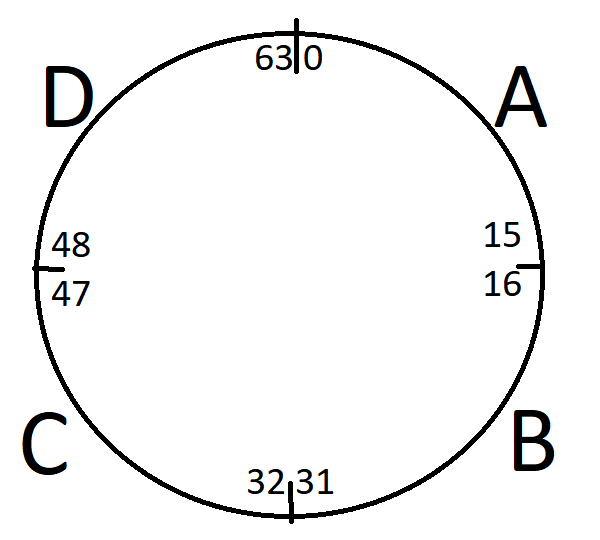
\includegraphics{fig/hashring.png}
    \caption{Eksempel på konsistent hashring i Project Voldemort.}
    \label{fig4}
\end{figure}

Den logiske strukturen til likemannsnettverket av databasenoder i Voldemort har formen til en ring. Denne ringen består av en stor mengde diskrete posisjoner, verdiområdet til en hashfunksjon \emph{h}. Hver node som deltar i databaseklyngen, tildeles en gruppe av disse punktene i ringen. \emph{h} brukes til å finne ringposisjonen til en nøkkel \emph{k}. Den noden, hvis tilordnede mengde av hashverdier inneholder \emph{h(k)}, blir den som lagrer det assosierte dataobjektet til \emph{k}.

Den konsistente hashalgoritmen og ringstrukturen til likemannsnettverket realiserer datareplikering ved å legge antallet påkrevde replikaer, per quorumkonfigurasjonen, på etter-følgende noder i ringen, med sola \citep{elmasri2014}. Per figur \ref{fig4} og replikakonfigurasjonen \(N=3\) vil eksempelvis alle dataobjekter som hashes til node A, også kopieres til node B og C. Av denne figuren kan man lese at node A lagrer nøkler med hashverdi 0-15, B lagrer nøkler hvis hashverdi er mellom 16 og 31, C lagrer nøkler hvis hashverdi er mellom 32 og 47, og D lagrer nøkler hvis hashverdi er mellom 48 og 63.



\cleardoublepage

% Hovedkjelder: sadalage2013; pensum fra egne fag

